% Options for packages loaded elsewhere
\PassOptionsToPackage{unicode}{hyperref}
\PassOptionsToPackage{hyphens}{url}
%
\documentclass[
]{article}
\usepackage{amsmath,amssymb}
\usepackage{iftex}
\ifPDFTeX
  \usepackage[T1]{fontenc}
  \usepackage[utf8]{inputenc}
  \usepackage{textcomp} % provide euro and other symbols
\else % if luatex or xetex
  \usepackage{unicode-math} % this also loads fontspec
  \defaultfontfeatures{Scale=MatchLowercase}
  \defaultfontfeatures[\rmfamily]{Ligatures=TeX,Scale=1}
\fi
\usepackage{lmodern}
\ifPDFTeX\else
  % xetex/luatex font selection
\fi
% Use upquote if available, for straight quotes in verbatim environments
\IfFileExists{upquote.sty}{\usepackage{upquote}}{}
\IfFileExists{microtype.sty}{% use microtype if available
  \usepackage[]{microtype}
  \UseMicrotypeSet[protrusion]{basicmath} % disable protrusion for tt fonts
}{}
\makeatletter
\@ifundefined{KOMAClassName}{% if non-KOMA class
  \IfFileExists{parskip.sty}{%
    \usepackage{parskip}
  }{% else
    \setlength{\parindent}{0pt}
    \setlength{\parskip}{6pt plus 2pt minus 1pt}}
}{% if KOMA class
  \KOMAoptions{parskip=half}}
\makeatother
\usepackage{xcolor}
\usepackage[margin=1in]{geometry}
\usepackage{longtable,booktabs,array}
\usepackage{calc} % for calculating minipage widths
% Correct order of tables after \paragraph or \subparagraph
\usepackage{etoolbox}
\makeatletter
\patchcmd\longtable{\par}{\if@noskipsec\mbox{}\fi\par}{}{}
\makeatother
% Allow footnotes in longtable head/foot
\IfFileExists{footnotehyper.sty}{\usepackage{footnotehyper}}{\usepackage{footnote}}
\makesavenoteenv{longtable}
\usepackage{graphicx}
\makeatletter
\def\maxwidth{\ifdim\Gin@nat@width>\linewidth\linewidth\else\Gin@nat@width\fi}
\def\maxheight{\ifdim\Gin@nat@height>\textheight\textheight\else\Gin@nat@height\fi}
\makeatother
% Scale images if necessary, so that they will not overflow the page
% margins by default, and it is still possible to overwrite the defaults
% using explicit options in \includegraphics[width, height, ...]{}
\setkeys{Gin}{width=\maxwidth,height=\maxheight,keepaspectratio}
% Set default figure placement to htbp
\makeatletter
\def\fps@figure{htbp}
\makeatother
\setlength{\emergencystretch}{3em} % prevent overfull lines
\providecommand{\tightlist}{%
  \setlength{\itemsep}{0pt}\setlength{\parskip}{0pt}}
\setcounter{secnumdepth}{5}
% !TEX TS-program = LuaLaTeX
%------------------------------- Preamble ------------------------------------------------------
%\documentclass[12pt,a4paper,english]{article} % document type and language

\usepackage{babel}   			% multi-language support
\usepackage{xcolor}			% text color
\usepackage{float}   				% floats
\usepackage{url}     				% urls
\usepackage{fontspec} 			% font
		\setmainfont{Calibri}
\usepackage{geometry} 		% margins
\usepackage{titlesec}			% section font size
		\titleformat*{\section}{\Large\bfseries}
		\titleformat*{\subsection}{\normalsize\itshape\bfseries}
\usepackage{polyglossia}		% Indent first paragraph in section
		\setmainlanguage{english}
		%\PolyglossiaSetup{english}{indentfirst=true} % wrong
		\SetLanguageKeys{english}{indentfirst=true}
\usepackage{titlesec}			% Format titles
		\titlespacing\section{0pt}{2pt plus 1pt minus 1pt}{0pt plus 1pt minus 1pt}
		\titlespacing\subsection{0pt}{2pt plus 1pt minus 1pt}{0pt plus 1pt minus 1pt}
		\titlespacing\subsubsection{0pt}{2pt plus 1pt minus 1pt}{0pt plus 1pt minus 1pt}
%\usepackage[none]{hyphenat}	% prevent word breaks


% Set up the fonts
%\usepackage[urw-palatino]{mathdesign}
%\usepackage[T1]{fontenc}


% Set the language for 508
\usepackage{hyperref}
\hypersetup{
  pdftitle = {title},
  pdflang = en-US}

% Add accessibility support from http://www.richschwinn.com/accessibility
\RequirePackage{accsupp}
\RequirePackage{pdfcomment}
\newcommand{\AccTool}[2]{\BeginAccSupp{method=pdfstringdef,unicode,Alt={{#1}}}\pdftooltip{{#2}}{{#1}}\EndAccSupp{}}


% Set up the headers and footers
\usepackage{graphicx}
\usepackage{fancyhdr}
\usepackage{ifthen}
%\usepackage{everypage-1x}
\usepackage{float}
%\usepackage{subfig}
%\usepackage{subcaption}

% Avoid struggling over figure and table float in Rmarkdown
\let\origfigure\figure
\let\endorigfigure\endfigure
\renewenvironment{figure}[1][2] {
    \expandafter\origfigure\expandafter[H]
} {
    \endorigfigure
}

\let\origtable\table
\let\endorigtable\endtable
\renewenvironment{table}[1][2] {
    \expandafter\origtable\expandafter[H]
} {
    \endorigtable
}

% First page has the large title and NOAA logo
%\pagestyle{fancy}
%\fancyhf{}
%\setlength\headheight{40pt}
%\fancyheadoffset[L]{0.5cm}
%\cfoot{\thepage}
%
%\fancyheadinit{%
%   \ifthenelse{\value{page}=4}%
%      {\fancyhead[R]{\includegraphics[width=40pt]{images/NOAA_logo.png} \\ \textsf{\emph{March 17, 2022}}}
%       \fancyhead[L]{\textsf{\LARGE State of the Ecosystem 2022: Mid-Atlantic}}
%      }%
%      {\fancyhead[R]{}
%       \fancyhead[L]{\textsf{\emph{State of the Ecosystem 2022: Mid-Atlantic}}}
%      }
%}



\renewcommand{\headrulewidth}{0.4pt}
\renewcommand{\footrulewidth}{0pt}

% Make caption fonts a bit smaller
\usepackage[font={small}]{caption}


% Change section labels to san serif
\usepackage{sectsty}
\allsectionsfont{\normalfont\sffamily\bfseries}

%\usepackage{lineno}
%\linenumbers

\usepackage{setspace}
\doublespacing
\usepackage{setspace}\onehalfspacing
\usepackage{float}
\usepackage{caption}
\captionsetup[figure]{labelformat=empty}
\usepackage{booktabs}
\usepackage{longtable}
\usepackage{array}
\usepackage{multirow}
\usepackage{wrapfig}
\usepackage{float}
\usepackage{colortbl}
\usepackage{pdflscape}
\usepackage{tabu}
\usepackage{threeparttable}
\usepackage{threeparttablex}
\usepackage[normalem]{ulem}
\usepackage{makecell}
\usepackage{xcolor}
\ifLuaTeX
  \usepackage{selnolig}  % disable illegal ligatures
\fi
\IfFileExists{bookmark.sty}{\usepackage{bookmark}}{\usepackage{hyperref}}
\IfFileExists{xurl.sty}{\usepackage{xurl}}{} % add URL line breaks if available
\urlstyle{same}
\hypersetup{
  pdftitle={Bluefin Combined Index Model V1},
  pdfauthor={Katie Lankowicz},
  hidelinks,
  pdfcreator={LaTeX via pandoc}}

\title{Bluefin Combined Index Model V1}
\author{Katie Lankowicz}
\date{30 June, 2023}

\begin{document}
\maketitle

{
\setcounter{tocdepth}{2}
\tableofcontents
}
\hypertarget{motivation}{%
\section{Motivation}\label{motivation}}

In the last several decades, global climate change has resulted in warming ocean temperatures and altered marine habitat suitability. Responses to these environmental changes can be seen at the individual, population, and ecosystem level for many marine fish species. Frequently, marine fish will shift their spatial-temporal distribution to track environmental conditions that are better-suited to their energetic requirements. It is suspected that the western stock of Atlantic Bluefin Tuna (BFT) is currently undergoing a climate-forced range shift due to rapidly warming conditions in the Northwest Atlantic. Recent stock assessments for BFT in US and Canadian waters have provided conflicting trends in catch-per-unit-effort (CPUE) indices for BFT, where the Canadian fishery has seen an increase in BFT CPUE and the American fishery has seen a decrease.

This project will create a joint CPUE index for BFT across American and Canadian waters in the Northwest Atlantic using Vector Autoregressive Spatio-Temporal (VAST) modeling. VAST is a flexible model framework based on delta-generalized linear mixed models, and is capable of incorporating information from multiple sources and gear types to create a joint index. VAST can also incorporate the effects of habitat and catchability covariates on organism spatio-temporal distribution. VAST outputs include spatial metrics including spatio-temporal density maps, hierarchical clustering of spatial areas based on organism density, stock center of gravity, area of utilization, and quantile of range edges.

The remainder of this document will be used to report progress on cleaning and merging American and Canadian BFT catch data and making VAST model structure decisions.

\hypertarget{bft-data-requirements}{%
\section{BFT data requirements}\label{bft-data-requirements}}

BFT data from American and Canadian fisheries are in variable formats and need to be heavily manipulated prior to merging. The goal is to create a dataframe where each row represents a sampling event. The following variables are desired for each sampling event:

\begin{itemize}
\tightlist
\item
  Unique trip identifier
\item
  Date
\item
  Spatial location (latitude and longitude, decimal degrees)
\item
  Number of hours spent fishing
\item
  Number of BFT caught in both large and small size groups
\item
  Sea surface temperature
\item
  Water depth
\item
  Sea level pressure
\item
  Basin-wide daily NAO index
\item
  Basin-wide monthly AMO index
\item
  Wind direction and velocity
\item
  Local chlorophyll-A concentration (as a proxy for plankton distribution)
\item
  Local prey biomass
\end{itemize}

\hypertarget{model-domains}{%
\subsection{Model domains}\label{model-domains}}

Currently, the model's temporal domain is 1993 - 2020. Though BFT total catch data were recorded prior to 1993, information to determine the size of each fish was not reliably recorded. The final model will include indices for multiple BFT size classes, and so data without associated length or weight information is not useful. The temporal domain currently ends at 2020 because that is the most recent year with Canadian catch data. American catch data ends at 2021. The temporal domain could be extended with new information.

The model spatial domain is the combined area of American and Canadian exclusive economic zones (EEZs) in the Northwest Atlantic, bounded on the south by Cape Hatteras, North Carolina and on the north by Cape North, Nova Scotia. The model does not consider the Gulf of Saint Lawrence, nor is any tuna catch data from that area included.

\begin{figure}
\centering
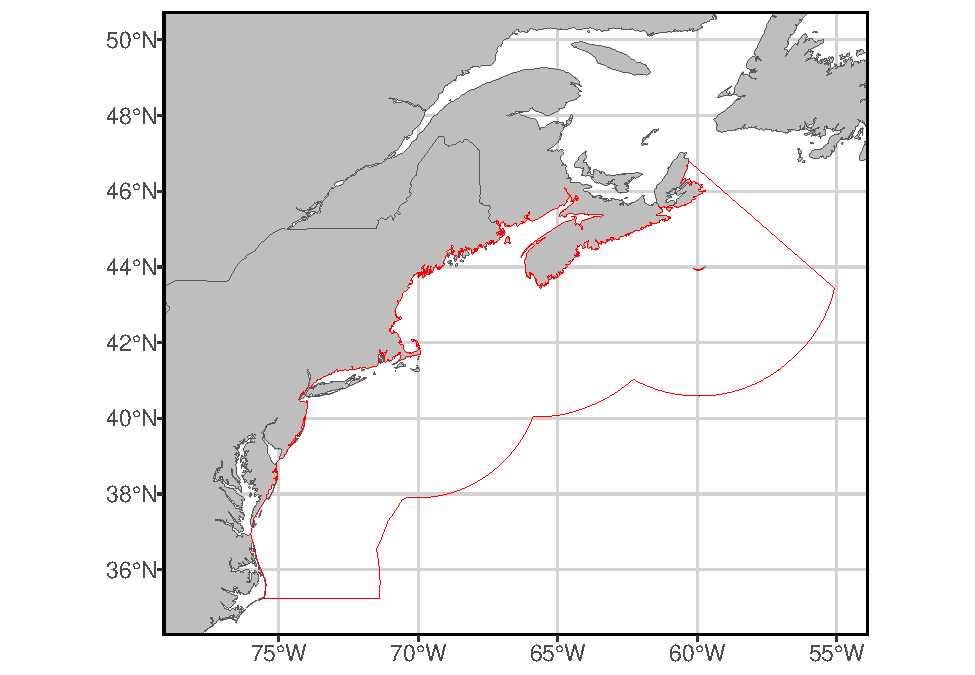
\includegraphics{Model_Prelim_Report_files/figure-latex/spatial-domain-1.pdf}
\caption{\label{fig:spatial-domain}Fig. 1: VAST model spatial domain}
\end{figure}

\hypertarget{bft-size-categories}{%
\subsection{BFT size categories}\label{bft-size-categories}}

BFT are categorized into six size classes by both weight and length. BFT migrations and habitat use are expected to vary with age, and so the ideal model will generate separate indices and spatial metrics for different age groupings. There is not enough information to do this for each of the six size classes, and so the size class information was pooled into two groupings: small and large. Small BFT are 144 cm (56.7 in) and shorter, while large BFT are longer than 177 cm (69.7 in). This structure was chosen to match the structure of current US handline BFT indices. Because the ``Small medium'' size class straddles the line between groups, these fish have been excluded from analysis.

BFT were categorized according to length, preferentially. If no length information was recorded, weight was used to categorize. If neither length nor weight information was recorded for a fish, it could not be included in analysis.

\begin{table}[H]

\caption{\label{tab:size-table}Bluefin tuna size classes}
\centering
\begin{tabular}[t]{lllll}
\toprule
Size class & Grouping & Curved Fork
Length & Pectoral Curved
Fork Length & Weight (lbs)\\
\midrule
Young school & Small & <27 in & <20 in & <14 lbs\\
School & Small & 27 - <47 in & 20 - <35 in & 14 - <66 lbs\\
Large school & Small & 47 - <59 in & 35 - <44 in & 66 - <135 lbs\\
Small medium & NA & 59 - <73 in & 44 - <54 in & 135 - <235 lbs\\
Large medium & Large & 73 - <81 in & 54 - <60 in & 235 - <310 lbs\\
\addlinespace
Giant & Large & 81+ in & 60+ in & 310+ lbs\\
\bottomrule
\end{tabular}
\end{table}

\hypertarget{us-bft-recreational-catch}{%
\subsection{US BFT Recreational Catch}\label{us-bft-recreational-catch}}

Catch and effort information for the US recreational BFT fishery is recorded by the Large Pelagics Survey, which is a dockside/telephone survey of a random sample of private and charter boat captains targeting large pelagics. We subset the full LPS dataset so only data from trips targeting BFT were included. Other filters were also applied: only tuna landed in Virginia and northwards were included, fishing trips needed to be between 1 and 24 hours in length, and only fishing trips ending on June 1st through October 31st of each year were included.

LPS data recording procedures changed in 2002, and so data are stored across two sets of files (1993-2002, 2002-present). These needed to be cleaned and merged. This process can be viewed in the accompanying RMarkdown document. An example of results will also be provided.

Note that sea surface temperature and water depth are not always provided by the anglers. We have merged these spatiotemporal catch data with NOAA 1/4° Daily Optimum Interpolation Sea Surface Temperature (OISST) and GEBCO 15 arc-second gridded bathymetric data to get complete data coverage for SST and depth.

\begin{landscape}\begin{table}[H]

\caption{\label{tab:mergelps}American Large Pelagic Survey example}
\centering
\begin{tabular}[t]{lrrrrrrrrrrrrr}
\toprule
Size & Trip
ID & Year & Month & Day & Hours
fished & Lon & Lat & nCatch & SST
(C) & Depth
(m) & Pressure & NAO & AMO\\
\midrule
large & 2 & 1993 & 10 & 1 & 6 & -71.36667 & 40.03333 & 0 & 19.65 & -6.7 & 102403 & 0.7010462 & -0.259\\
small & 3 & 1993 & 10 & 1 & 6 & -71.36667 & 40.03333 & 1 & 19.65 & -6.7 & 102403 & 0.7010462 & -0.259\\
large & 3 & 1993 & 10 & 1 & 6 & -71.36667 & 40.03333 & 0 & 19.65 & -6.7 & 102403 & 0.7010462 & -0.259\\
small & 2 & 1993 & 10 & 1 & 6 & -71.36667 & 40.03333 & 2 & 19.65 & -6.7 & 102403 & 0.7010462 & -0.259\\
large & 1 & 1993 & 10 & 2 & 9 & -70.50000 & 42.16667 & 0 & 13.62 & -5.2 & 101980 & 0.9867340 & -0.259\\
\addlinespace
small & 1 & 1993 & 10 & 2 & 9 & -70.50000 & 42.16667 & 10 & 13.62 & -5.2 & 101980 & 0.9867340 & -0.259\\
\bottomrule
\end{tabular}
\end{table}
\end{landscape}

\begin{figure}
\centering
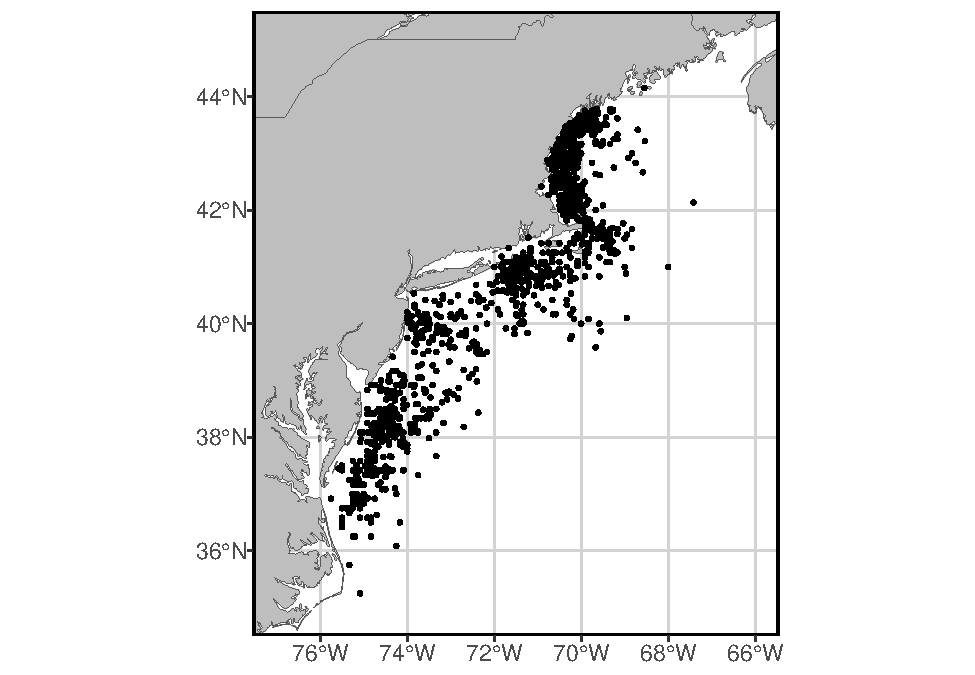
\includegraphics{Model_Prelim_Report_files/figure-latex/americanplot-1.pdf}
\caption{\label{fig:americanplot}Fig. 2: Spatial distribution of American recreational catch}
\end{figure}

\hypertarget{canadian-bft-commercial-landings}{%
\subsection{Canadian BFT Commercial Landings}\label{canadian-bft-commercial-landings}}

Catch and effort data for the Canadian commercial BFT fishery are recorded in commercial logbooks. We will only be working with commercial data from the Southwest Nova Scotia region, though data exists for the Gulf of Saint Lawrence region as well. The same data filters regarding fishing hours and month fished applied to the US data were applied to the Canadian data. Though the US recreational fishery is likely all rod and reel, the Canadian commercial fishery also includes harpoon and tended line gear. This could later inform some model structure decisions.

Data collection methods changed in 2003, and so the data are stored across two sets of files (Commercial Landings 95-03, Historical Data. These needed to be cleaned and merged. This process can be viewed in the accompanying RMarkdown document. An example of results will also be provided.

There are some concerns with the historic (1993-2002) Canadian data. The data have several columns that I cannot make sense of without metadata. Although I assume I have only been provided with BFT catch, there is a column for species landed in the data. The values within this column are numeric (252-256), and I do not know what these numbers mean. For now, I have made the assumption that all these species codes refer to BFT. In the future, I can subset out non-BFT data if I am made aware that some of these species codes are not BFT.

\begin{landscape}\begin{table}[H]

\caption{\label{tab:mergecan}Canadian commercial data example}
\centering
\begin{tabular}[t]{lrrrrrrrrrrrrr}
\toprule
Size & Trip
ID & Year & Month & Day & Hours
fished & nCatch & SST
(C) & Depth
(m) & Pressure & NAO & AMO & Lon & Lat\\
\midrule
large & 1 & 1993 & 10 & 1 & 8 & 0 & 15.42 & -165.0 & 102205 & 0.7010462 & -0.259 & -65.21667 & 42.96667\\
Unknown & 1 & 1993 & 10 & 1 & 8 & 10 & 15.42 & -165.0 & 102205 & 0.7010462 & -0.259 & -65.21667 & 42.96667\\
small & 1 & 1993 & 10 & 1 & 8 & 0 & 15.42 & -165.0 & 102205 & 0.7010462 & -0.259 & -65.21667 & 42.96667\\
small & 2 & 1993 & 10 & 2 & 8 & 0 & 15.77 & -378.1 & 102585 & 0.9867340 & -0.259 & -65.60000 & 42.05000\\
large & 2 & 1993 & 10 & 2 & 8 & 0 & 15.77 & -378.1 & 102585 & 0.9867340 & -0.259 & -65.60000 & 42.05000\\
\addlinespace
Unknown & 2 & 1993 & 10 & 2 & 8 & 2 & 15.77 & -378.1 & 102585 & 0.9867340 & -0.259 & -65.60000 & 42.05000\\
\bottomrule
\end{tabular}
\end{table}
\end{landscape}

\begin{figure}
\centering
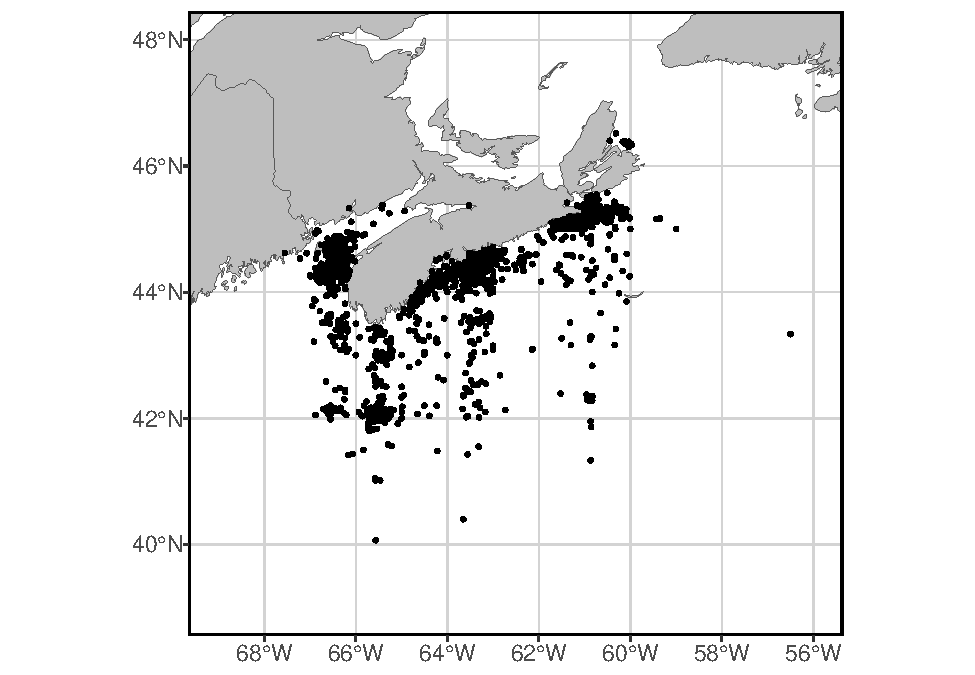
\includegraphics{Model_Prelim_Report_files/figure-latex/canadianplot-1.pdf}
\caption{\label{fig:canadianplot}Fig. 3: Spatial distribution of Canadian commercial catch}
\end{figure}

\hypertarget{model-structure}{%
\section{Model structure}\label{model-structure}}

\hypertarget{response-variable-and-effort-adjustment}{%
\subsection{Response variable and effort adjustment}\label{response-variable-and-effort-adjustment}}

\hypertarget{spatial-temporal-spatio-temporal-variation}{%
\subsection{Spatial, Temporal, Spatio-temporal variation}\label{spatial-temporal-spatio-temporal-variation}}

\hypertarget{density-covariates}{%
\subsection{Density covariates}\label{density-covariates}}

\hypertarget{preliminary-results}{%
\section{Preliminary results}\label{preliminary-results}}

\end{document}
